\documentclass[11pt]{article}
\usepackage[margin=0.7in]{geometry}
\usepackage{multirow}
\usepackage {graphicx}
\usepackage[utf8x]{inputenc} % указать кодировку русского текста
\usepackage[russian]{babel} % указать, что язык текста - русский
\usepackage{fancyhdr}
\pagestyle{fancy}
\usepackage{graphicx}
\graphicspath{{pictures/}}
\DeclareGraphicsExtensions{.pdf,.png,.jpg}
\usepackage{tocloft}
\renewcommand{\cftsecleader}{\cftdotfill{\cftdotsep}}
\begin{document}
\begin{titlepage}
\begin{center}
\large\textbf{Московский Физико-Технический Институт}\\
\large\textbf{(государственный университет)}
\vfill
\huge\textbf{ Работа 3.4.2}\\
\huge\textbf{Закон Кюри-Вейсса}\\
\vfill
\large Факультет электроники, фотоники и молекулярной физики\\
\end{center}
\end{titlepage}
\fancyhead[L] {Работа 3.4.2}
\tableofcontents
\newpage
\textbf{Цель работы:}\\
 Изучение температурной зависимости магнитной воприимчивости ферромагнетика выше точки Кюри.

\textbf{В работе используются:}\\
 Катушка самоиндукции с образцом из гадолиния, термостат, частотометр, цифровой вольтметр, LC-автогенератор, термопара медь-константан.


\section{Теоретическая часть}
	Вещества с отличными от нуля атомными магнитными моментами обладают парамагнитными свойствами. Внешнее магнитное поле оринетирует магнитные моменты, которые в отсуствие поля располагались в пространстве хаотическим образом. Однако при $T \rightarrow 0$ тепловое движение всё меньше препятствует магнитным моментам атомов оринетироваться в одном направлении при сколь угодно слабом внешнем поле. В ферромагнетиках -- под влиянием обменных сил -- это происходит при понижении температуры не до абсолютного нуля, а до температуры Кюри $\Theta$. Оказывается, что у ферромагнетиков магнитная восприимчивость должна удовлетворять закону Кюри-Вейсса:
	\begin{equation}
		\label{eq:Kuri-Veicca}
		\chi \propto \frac{1}{T-\Theta_p},
	\end{equation}
	где $\Theta_p$ -- температура, близкая к температуре Кюри, так как при $T \approx \Theta$ формула~(\ref{eq:Kuri-Veicca}) недостаточна точна.
\section{Экспериментальная установка}
	Схема установки для проверки закона Кюри-Вейсса показана на рис.~\ref{ris:ustanovka}. Исследуемый ферромагнитный образец (гадолиний) расположен внутри пустотелой катушки самоиндукции, которая служит инудктивностью колебательного конутра, входящего в состав LC-автогенератора. Автогенератор собран на полевом транзисторе КП-103 и смонитрован в виде отдельного блока.\\
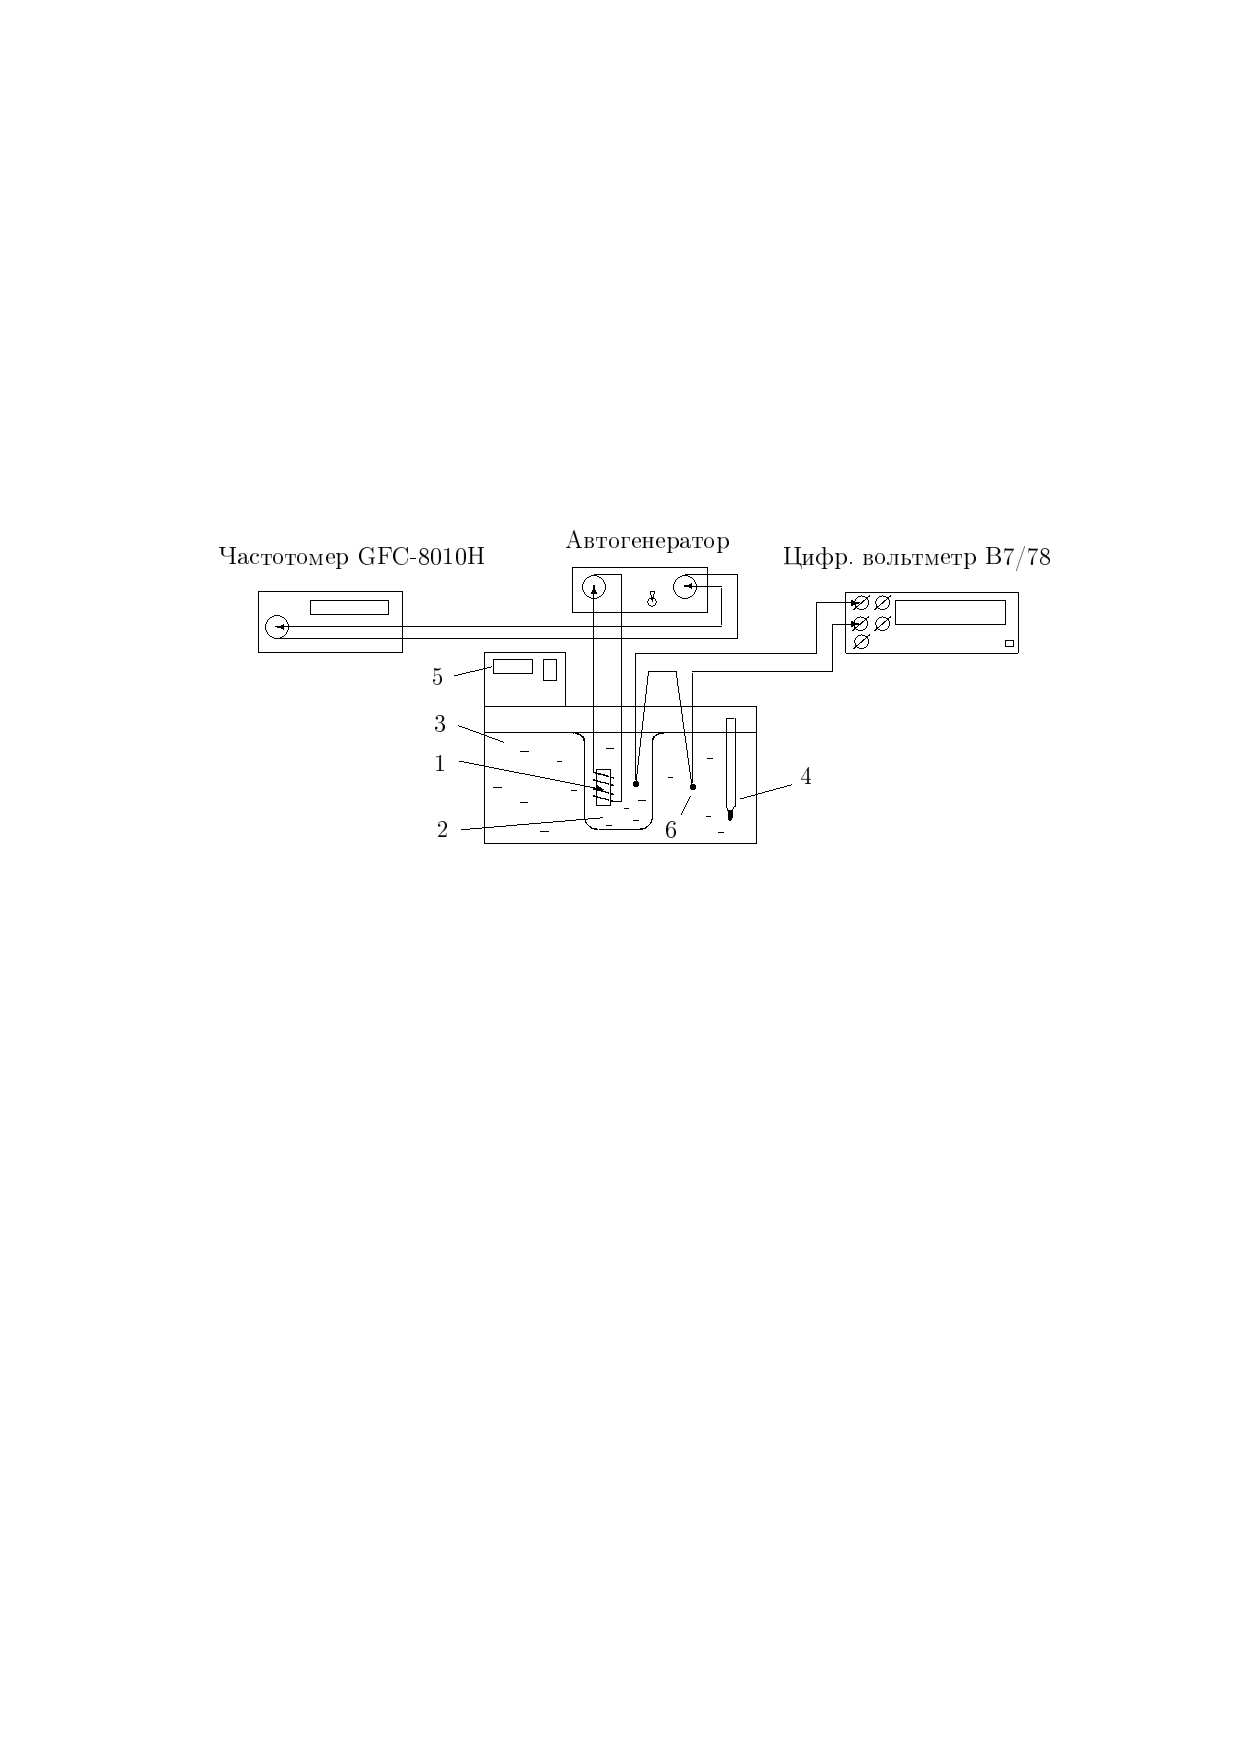
\includegraphics[scale=1]{ustanovka.pdf}\\
	Магнитная воосприимчивость образца $\chi$ определяется по изменению самоиндукции катушки. Обозначив через $L$ самоиндукцию катушки с образцом и через $L_0$ -- её самоиндукцию в отсутствие образца, получим
		$$(L-L_0)\propto \chi$$
При изменении самоиндукции образца меняется период колебаний автогенератора:
		$$\tau = 2\pi \sqrt{LC}$$
	где $C$ -- ёмкость конутра автогенератора. Период колебаний в отсуствие образца опредлеяется самоиндукцией пустой катушки:
		$$\tau_0 = 2\pi \sqrt{L_0C}$$
Отсюда находим:
$$(L-L_0)\propto \tau^2 - \tau_{0}^2$$
и,следовательно,
$$\chi \propto  \tau^2 - \tau_{0}^2$$
Итак, закон Кюри-Вейсса справедлив, если выполнено соотношение:
		$$\frac{1}{\chi} \propto (T-\Theta_p) \propto \frac{1}{\tau^2-\tau_0^2}$$

\section{Экспериментальные данные}
Константа термопары $k = 24$ град/мв\\
$\tau_{0} = 6,9092$ мкс - период колебаний в отсутствие образца.
\section{Ход работы}
\subsection{Измерение величин, необходимых для вычисления температуры Кюри}
17.11.21
Лаба огонь. точнее лед
Сенсей\\

Константа термопары $k = 24$ град/мв, поэтому ЭДС при допустимой $\triangle T = 0,5$ градусов Цельсия не должна превышать $\frac{\triangle T}{k} \approx 0,021$ мВ.\\
Исследуем зависимость периода колебаний $\tau$ по частотометру, а температуру $T$ - по показаниям дисплея и цифровому вольтметру ($T = T_{display} + k\times \triangle U$), учитывая знак ЭДС (термопара подключена так, что при знаке "+" на табло вольтметра температура образца выше температуры рабочей жидкости).\\
Диапазон измерений $13 \div 41$ градусов цельсия;\\
Данные измерений приведены в таблице:\\
\\
\begin{tabular}{|l|l|l|l|l|l|}
\hline
$T_{display}$ & $\tau$ & $\triangle U$& $\tau^2 - \tau^2_{0}$  & $T$ & $\frac{1}{\tau^2 - \tau^2_{0}}$\\
\hline
$\sigma_{T} = 0,01$ &  $\sigma_{\tau} = 0,0005$ мкс & $\sigma_{\triangle U} = 0,0005$ мВ &$\sigma_{\tau^2 - \tau_{0}^2} = 0,007$ мкс & $\sigma_{T} \approx 0,84$ г.Ц & $\sigma{\frac{1}{\tau^2 - \tau_{0}^2}} = 0,0047$ \\
\hline
13,08 & 7,968 & -0,016 & 15,7519 & 12,696 & 0,0634\\
\hline
15,05 & 7,934 & -0,018 & 15,2113 & 14,618 & 0,0657\\
\hline
17,04 & 7,863 & -0,017 & 14,0897 & 16,632 & 0,0709\\
\hline
19,06 & 7,735 & -0,015 & 12,0931 & 18,7 & 0,0827\\
\hline
21,08 & 7,54 & -0,014 & 9,1145 & 20,744 & 0,1097\\
\hline
23,04 & 7,369 & -0,018 & 6,5661 & 22,608 & 0,1523\\
\hline
25,03 & 7,207 & -0,019 & 4,2038 & 25,486 & 0,2379\\
\hline
27,04 & 7,139 & -0,018 & 3,2283 & 26,608 & 0,3098\\
\hline
29,05 & 7,1 & -0,017 & 2,6729 & 28,642 & 0,3741\\
\hline
31,05 & 7,075 & -0,015 & 2,3186 & 30,69 & 0,4313\\
\hline
33,04 & 7,058 & -0,014 & 2,0783 & 32,704 & 0,4811\\
\hline
35,02 & 7,045 & -0,017 & 1,8949 & 34,612 & 0,5277\\
\hline
37,01 & 7,036 & -0,017 & 1,7682 & 36,602 & 0,5655\\
\hline
39,01 & 7,028 & -0,016 & 1,6557 & 38,626 & 0,6039\\
\hline
41,04 & 7,022 & -0,014 & 1,5714 & 40,704 & 0,6363\\
\hline

\end{tabular}\\
\\
\subsection{Расчёт погрешностей}
Приведем расчёт погрешностей вычисления последних трёх величин:\\
1) $ T = T_{display} + k\times \triangle U$\\
$(\frac{\sigma_T}{T})^2 = (\frac{\sigma_{T_{display}}}{T_{display}})^2 + (k \times \frac{\sigma_{\triangle U}}{\triangle U})^2$\\
Суммируем и усредняем каждую переменную, чтобы найти среднее значение:\\
$(\frac{\sigma_T}{T})^2 = (\frac{0,01}{27,04})^2 + (\frac{0,0005}{-0,016})^2 \approx 1,367\cdot 10^{-7} + 0,097 \approx 0,00097$\\
$\sigma_{T} \approx 0,03 \cdot 27,04 \approx 0,84$\\
\fbox{$\sigma_{T} \approx 0,84$ г.Ц}\\

2) $\sigma_{\tau^2 - \tau_{0}^2} = \frac{d(\tau^2 - \tau_{0}^2)}{d\tau}\sigma_{\tau} = 2\tau\sigma_{\tau}$\\
\fbox{$\sigma_{\tau^2 - \tau_{0}^2} = 0,007$ мкс}\\
3) $\sigma{\frac{1}{\tau^2 - \tau_{0}^2}} = \frac{d(\frac{1}{\tau^2 - \tau_{0}^2})}{d\tau}\sigma_{\tau} = \frac{2\tau \sigma_\tau}{(\tau^2 - \tau_{0}^2)^2}$\\
\fbox{$\sigma{\frac{1}{\tau^2 - \tau_{0}^2}} = 0,0047$}\\
\subsection{График экспериментальной зависимости}
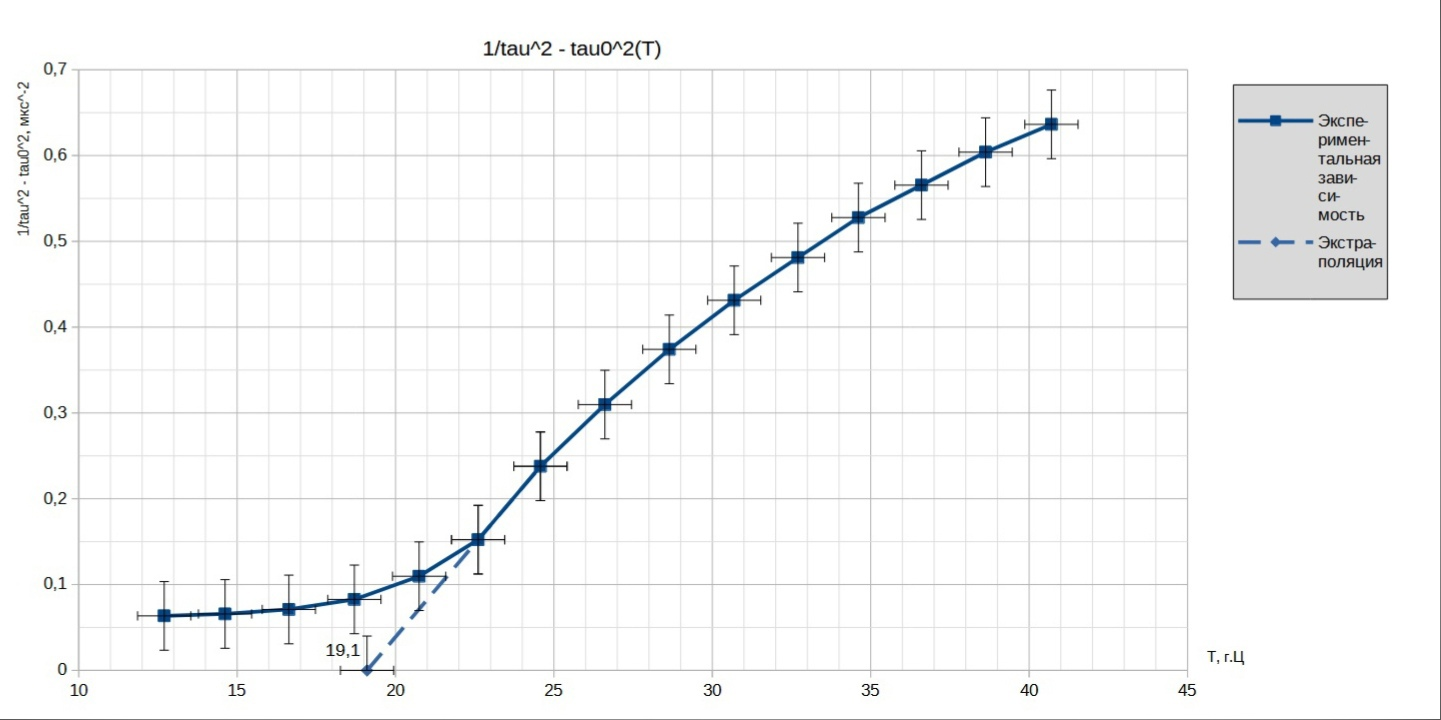
\includegraphics[width= 20cm]{g1}\\
Экстраполируя полученную прямую к оси абсцисс, определим парамагнитную точку Кюри $\theta_{p}$ для гадолиния.\\
\fbox {$\theta_{p} = 19,1$ г.Ц}\\
Расчёт и построение прямой:\\
$ y = a + bx$\\
$ 0,1523 = a +22,608b$\\
$ 0,2378 = a + 24,574b$\\
Таким образом, коэффициенты прямой:\\
\begin{tabular}{|l|l|}
\hline
a & b\\
\hline
-0,8311 & 0,0435\\
\hline
$\sigma_{a} = 0,09$ & $\sigma_{b} = 0,005$\\
\hline
\end{tabular}\\
\\
Погрешность полученной величины:\\
$\sigma_{\theta_{p}} = \theta_{p}\sqrt{(\frac{\sigma_{a}}{a})^2 + (\frac{\sigma_{b}}{b})^2} \approx 19,1\sqrt{0,0117 + 0,0132} \approx 3,1178 \approx 3,1$\\
Тогда \fbox{$\theta_{p} = 19,1 \pm 3,1$ г.Ц}\\
Табличное значение для гадолиния: $\theta_{t} = 20,2$ г.Ц\\
Поэтому полученный экспериментально результат имеет погрешность $5\%$\\
\section{Вывод}
По результатам проделанной работы мы получили парамагнитную точку Кюри для гадолиния. Её значение $\theta_{p} = 19,1 \pm 3,1$ г.Ц. Расхождение с теоретическим значением - $\theta_{t} = 20,2$ - составило $5\%$.\\
Как и предполагалось в теоретическом сведении, эта точка выше обычной точки Кюри, которая равна примерно 16 - 17 градусов.\\
Оценить обычную точку Кюри не удалось из-за специфики графика.\\
\end{document}